\chapter{Continuous Delivery}
Met TravisCI kun je ook continuous delivery regelen, op de Travis worden verschillende providers genoemd.

\begin{figure}[H]
	\centering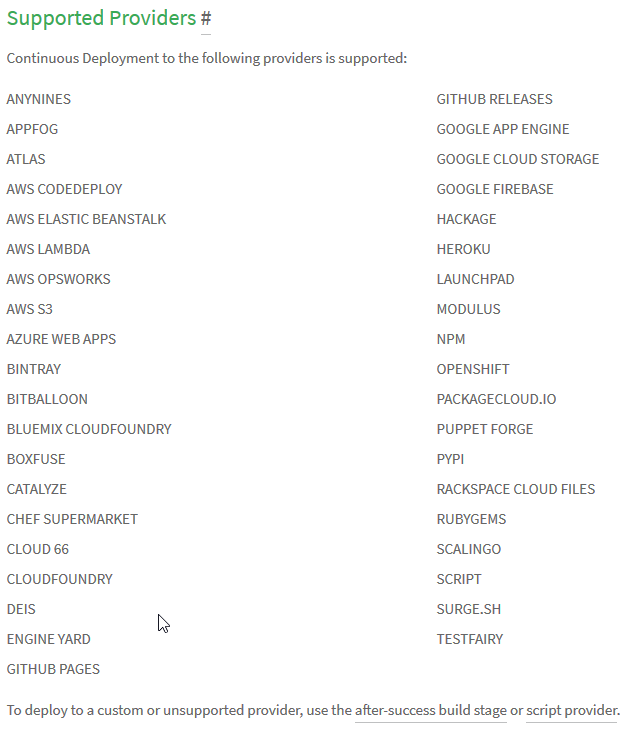
\includegraphics[width=0.35\textwidth]{images/TravisCICDProviders}
	\caption{Providers met support in TravisCI}
\end{figure}
Het deployen van applicaties gebeurt ook via de .travis.yml.
Omdat de .travis.yml file publiekelijk toegangkelijk is, is er ook de mogelijkheid om de wachtwoorden van verschillende services encrypted in de file te zetten.
Deze encryptie moet ervoor zorgen dat anderen niet zomaar op jouw account acties kunnen uitvoeren.

\section{Deployment}
Deployment wordt gergeld via eigen servers op het infralab van Fontys.
Omdat de applicatie op JavaEE gebouwd is moet de applicatie gedeployed worden op een applicatieserver.
Voor deze applicatieserver is Wildfly gekozen, een applicatieserver voor JBOSS JavaEE based applicaties.
Met Wildfly kunnen applicaties gedeployed worden met een console commando.